

\begin{figure}[hbtp]
\centering
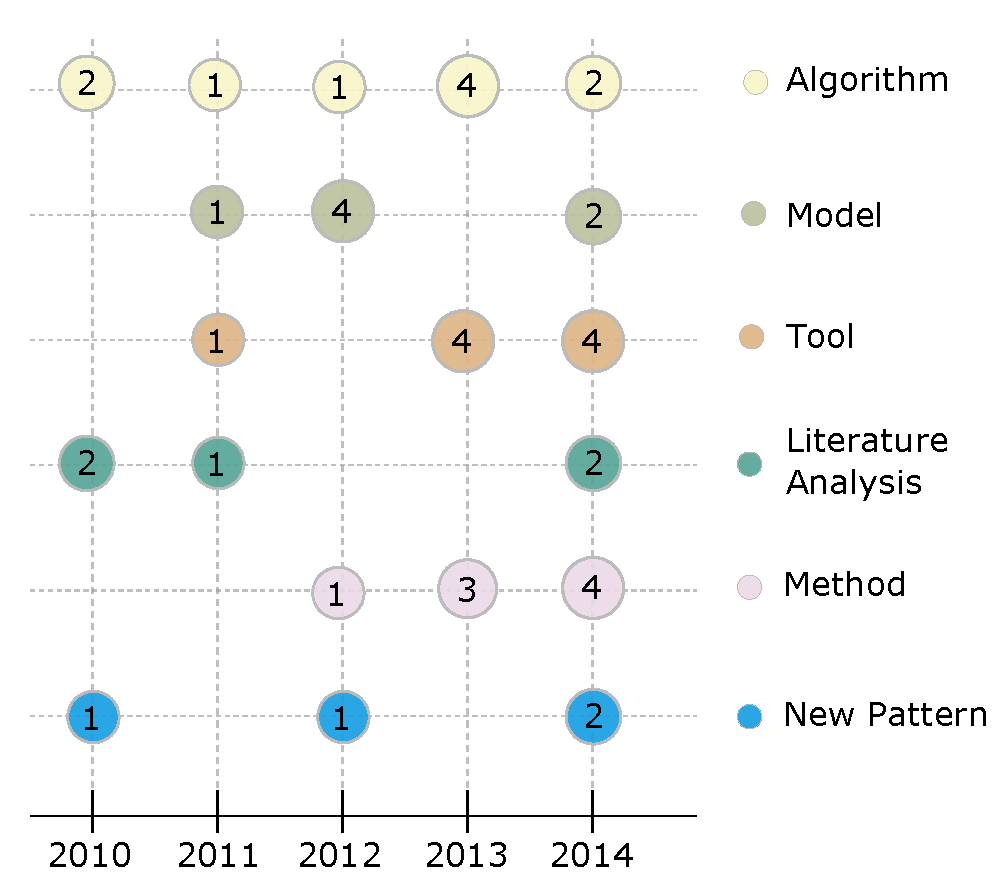
\includegraphics[width=0.79\textwidth]{figs/ContributionPerYear.pdf}
\caption{Contribution per year}
\label{fig:contribution-per-year}
\end{figure}

\begin{figure}[hbtp]
\centering
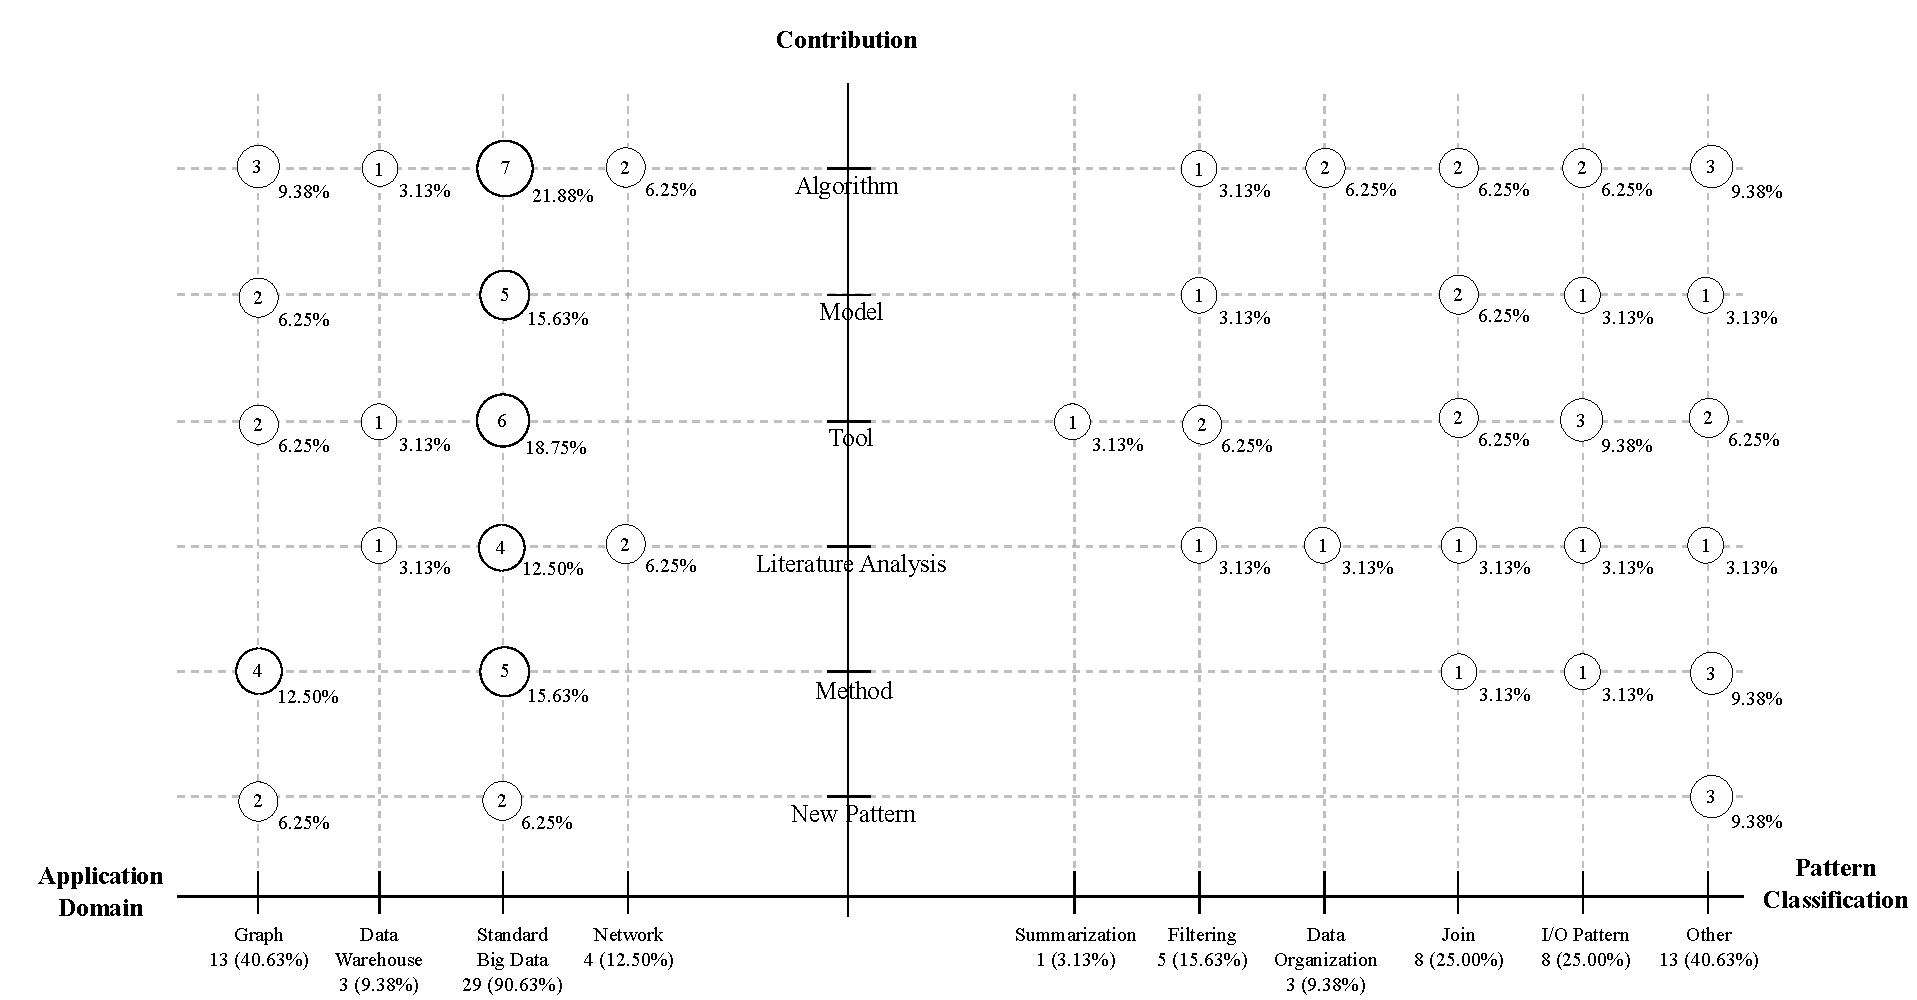
\includegraphics[width=0.99\textwidth]{figs/Contribution-Patterns-Domain.pdf}
\caption{Facet Contribution being related with the facets Pattern
Classification and Application Domain}
\label{fig:contribution-patterns-domain}
\end{figure}

\begin{figure}[hbtp]
\centering
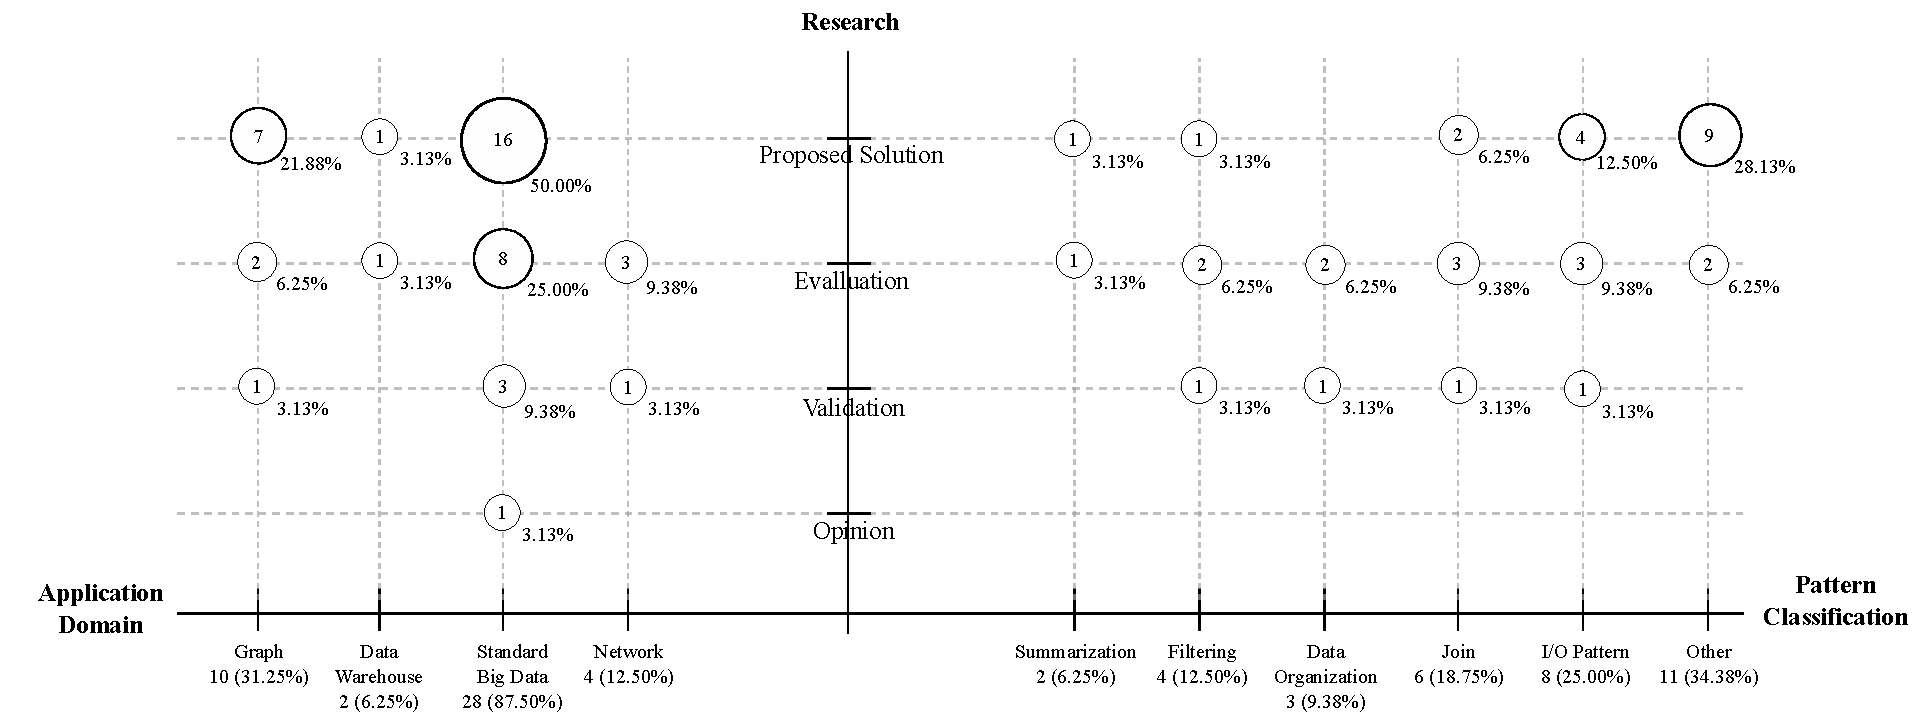
\includegraphics[width=0.99\textwidth]{figs/Research-Patterns-Domain.pdf}
\caption{Facet Research being related with the facets Pattern
Classification and Application Domain}
\label{fig:research-patterns-domain}
\end{figure}

\begin{figure}[hbtp]
\centering
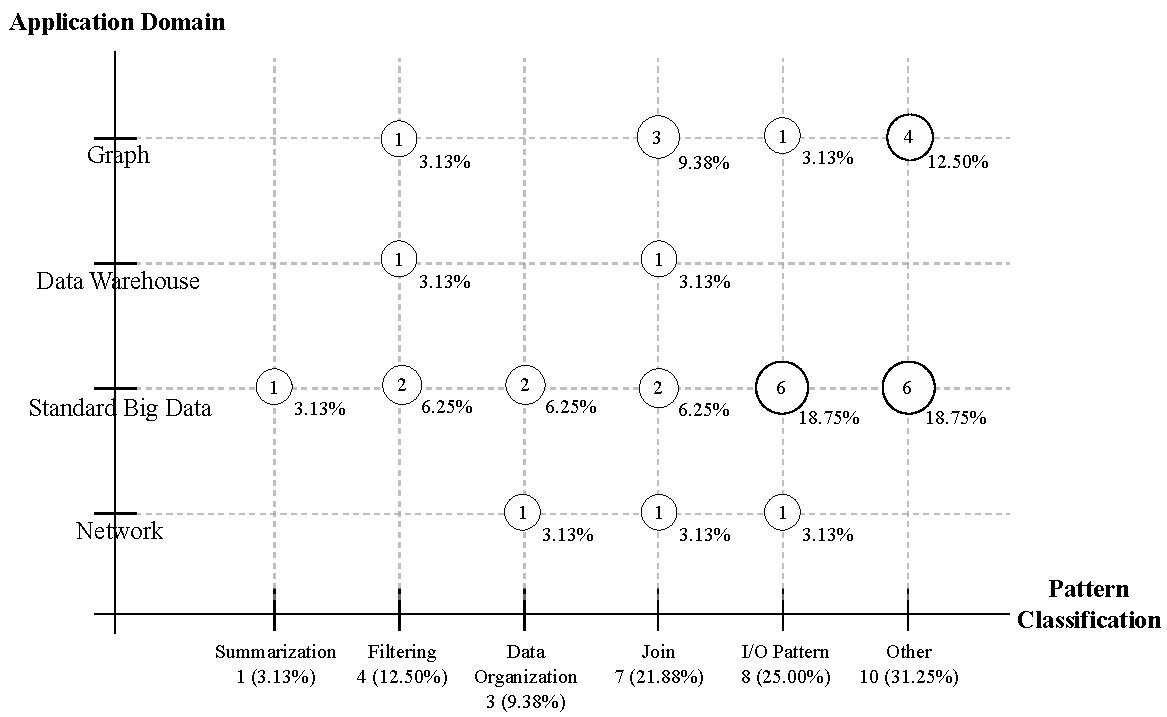
\includegraphics[width=0.99\textwidth]{figs/Patterns-Domain.pdf}
\caption{Facets Pattern
Classification and Application Domain relationship}
\label{fig:patterns-domain}
\end{figure}
          
   \begin{figure}[ht!]
 \centering 
  \subfloat[\textit{Ebooks} Data]
  {\label{fig:pisp6}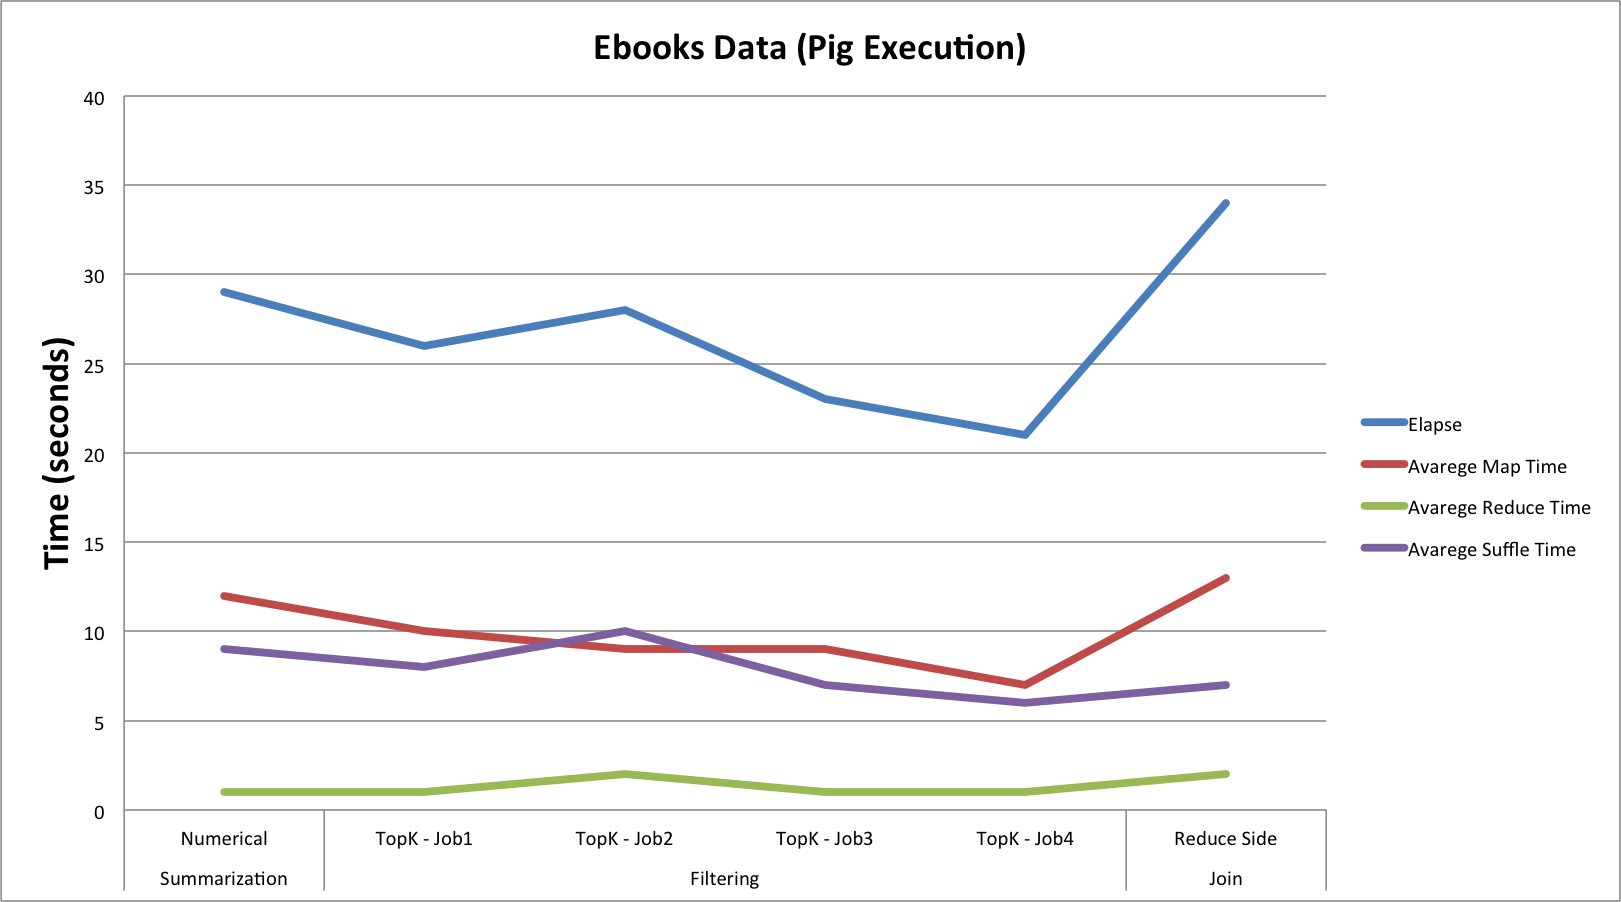
\includegraphics[width=0.471\textwidth]{figs/analysis-charts/pig/ebooks.png}}   
  \subfloat[\textit{Tex} Data]
  {\label{fig:pisp7}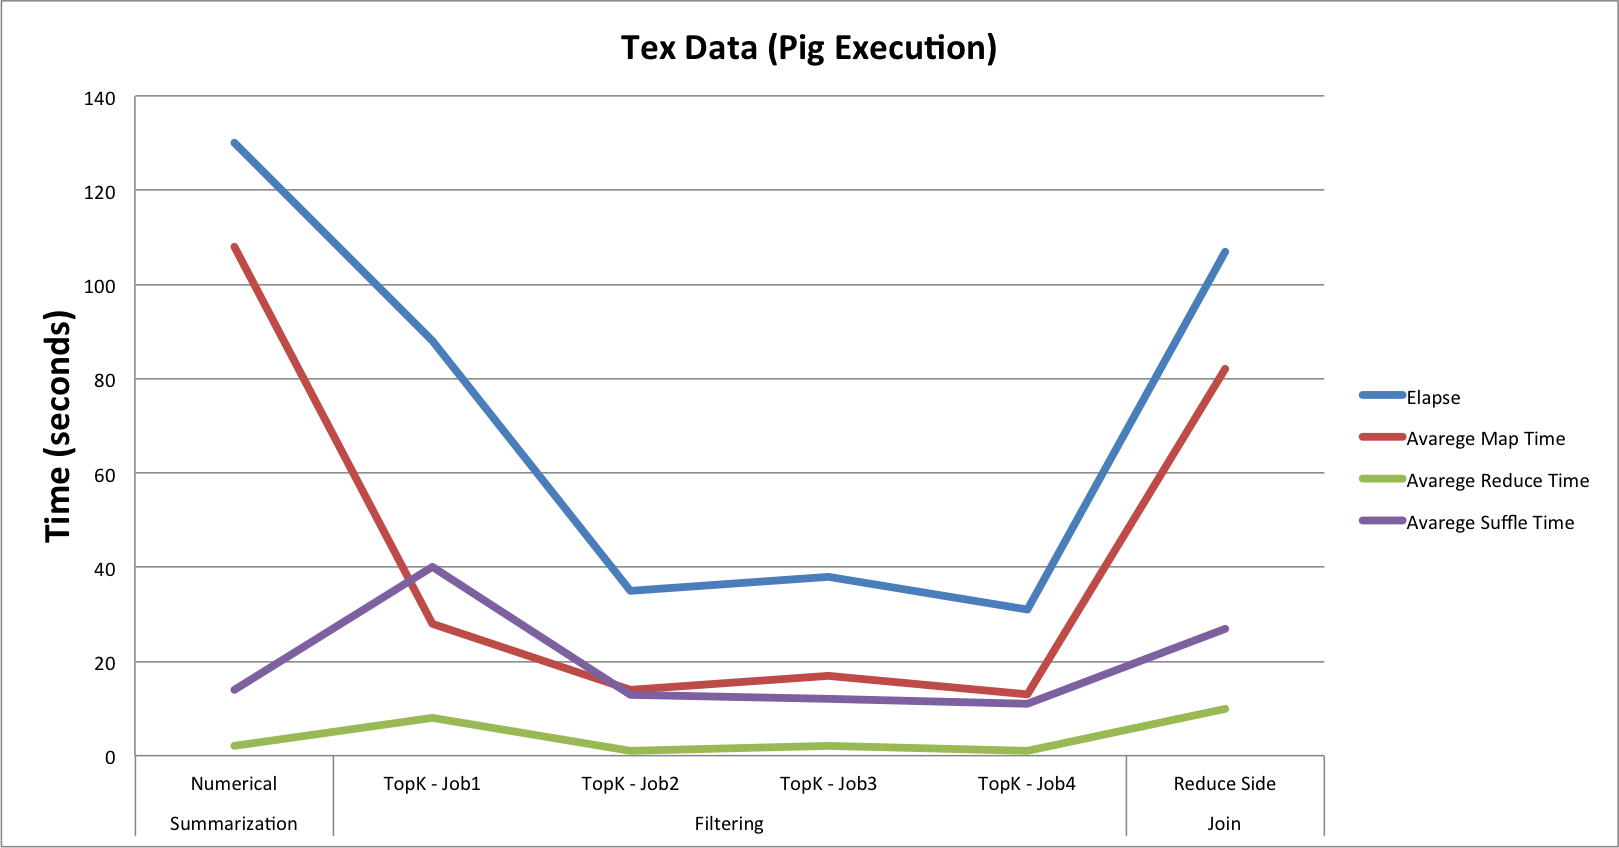
\includegraphics[width=0.5\textwidth]{figs/analysis-charts/pig/tex.png}}
   %add desired spacing between images, e. g. ~, \quad, \qquad etc. (or a blank line to force the subfig onto a new line)
  %~
  \\
  \subfloat[\textit{Serverfault} Data]
  {\label{fig:pisp6}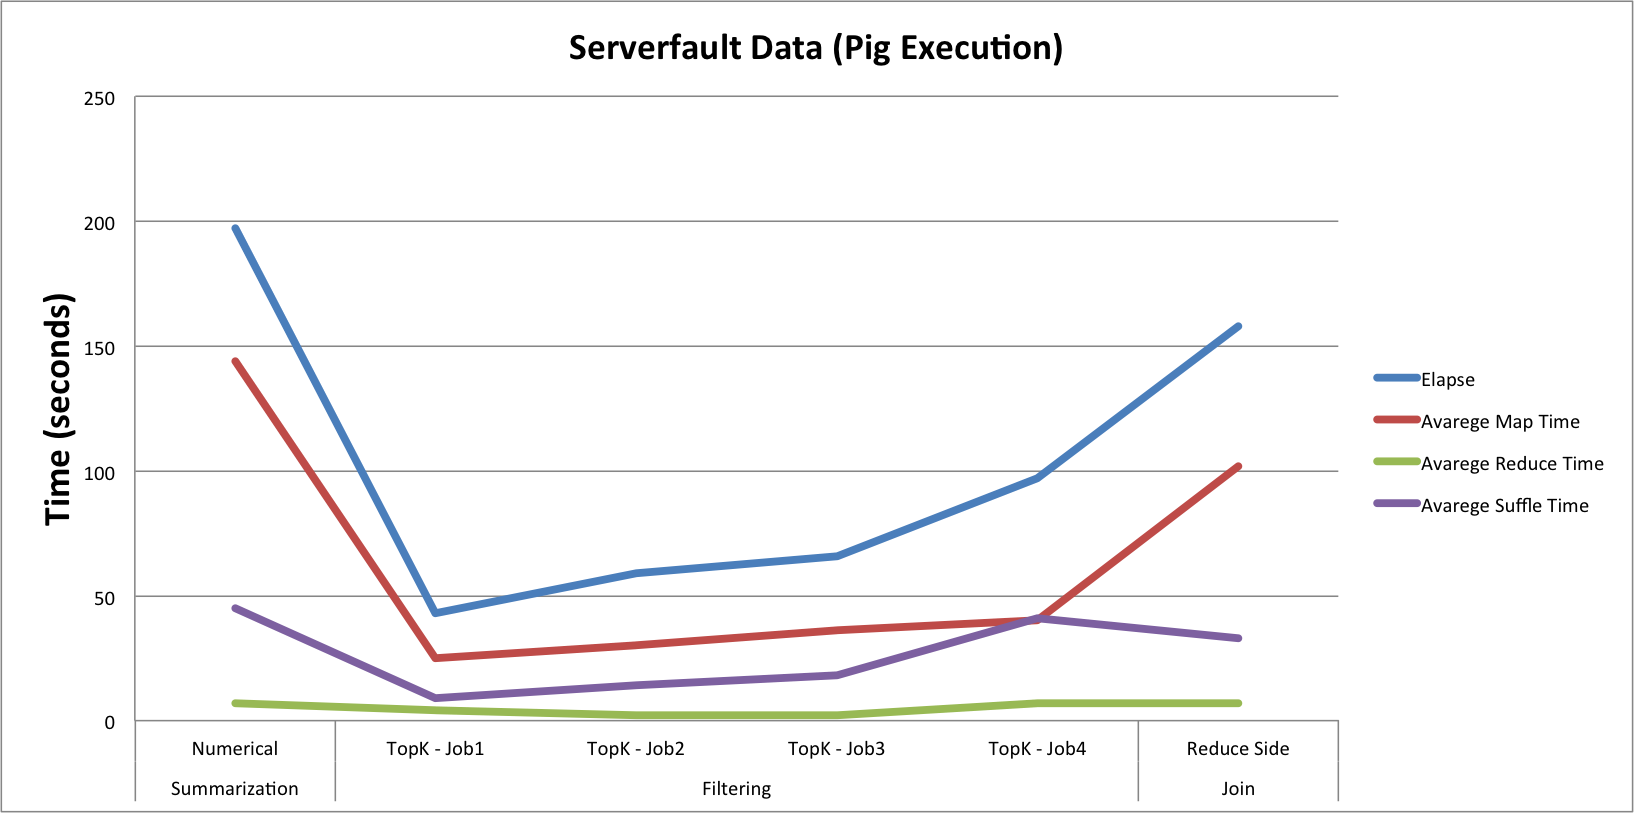
\includegraphics[width=0.5\textwidth]{figs/analysis-charts/pig/serverfault.png}}   
  \subfloat[\textit{Wordpress} Data]
  {\label{fig:pisp7}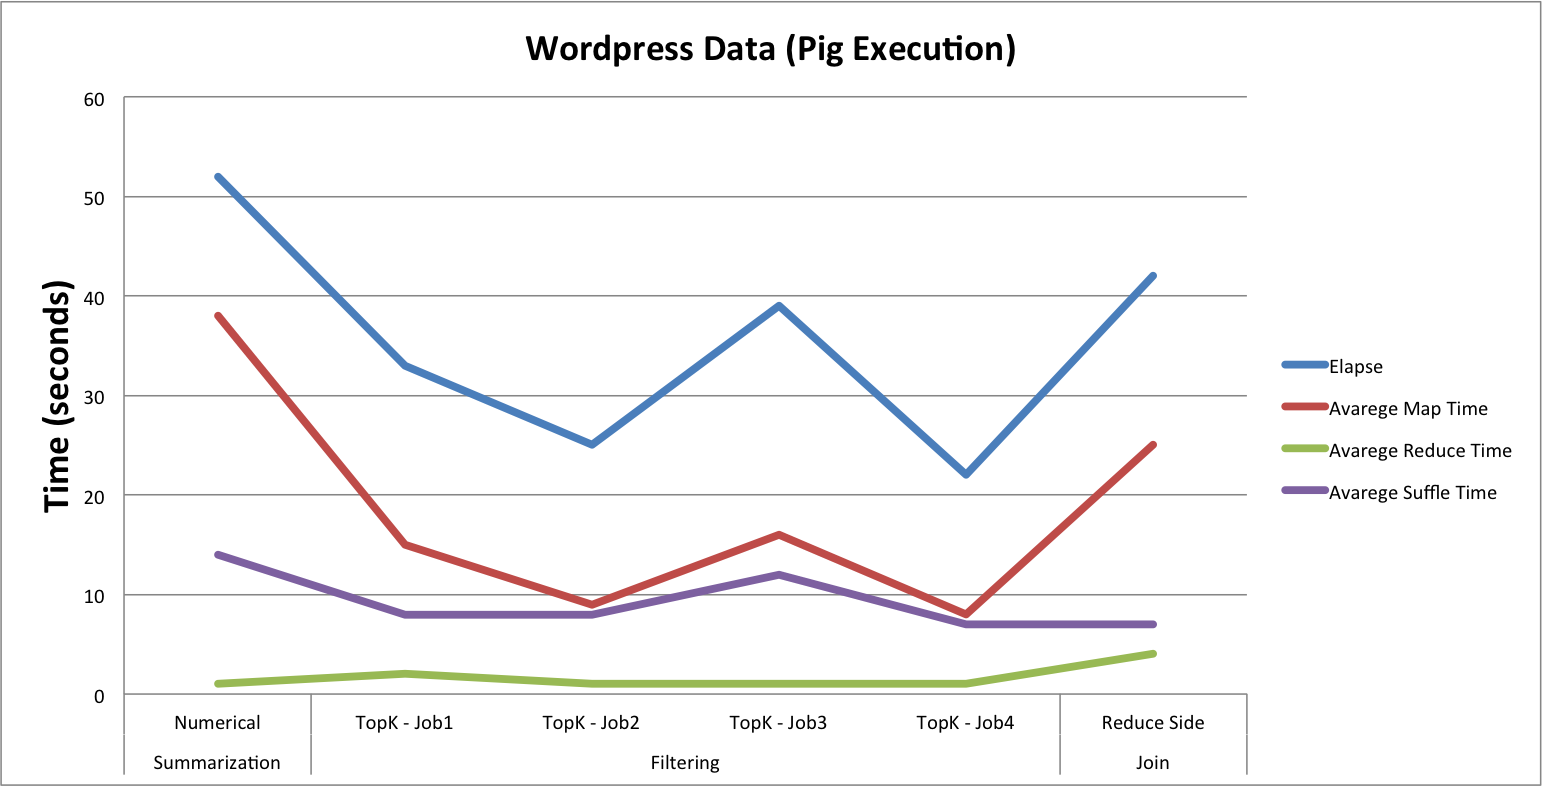
\includegraphics[width=0.49\textwidth]{figs/analysis-charts/pig/wordpress.png}}
   %add desired spacing between images, e. g. ~, \quad, \qquad etc. (or a blank line to force the subfig onto a new line)
  %~
  \\
  \subfloat[\textit{Webapps} Data]
  {\label{fig:pisp8}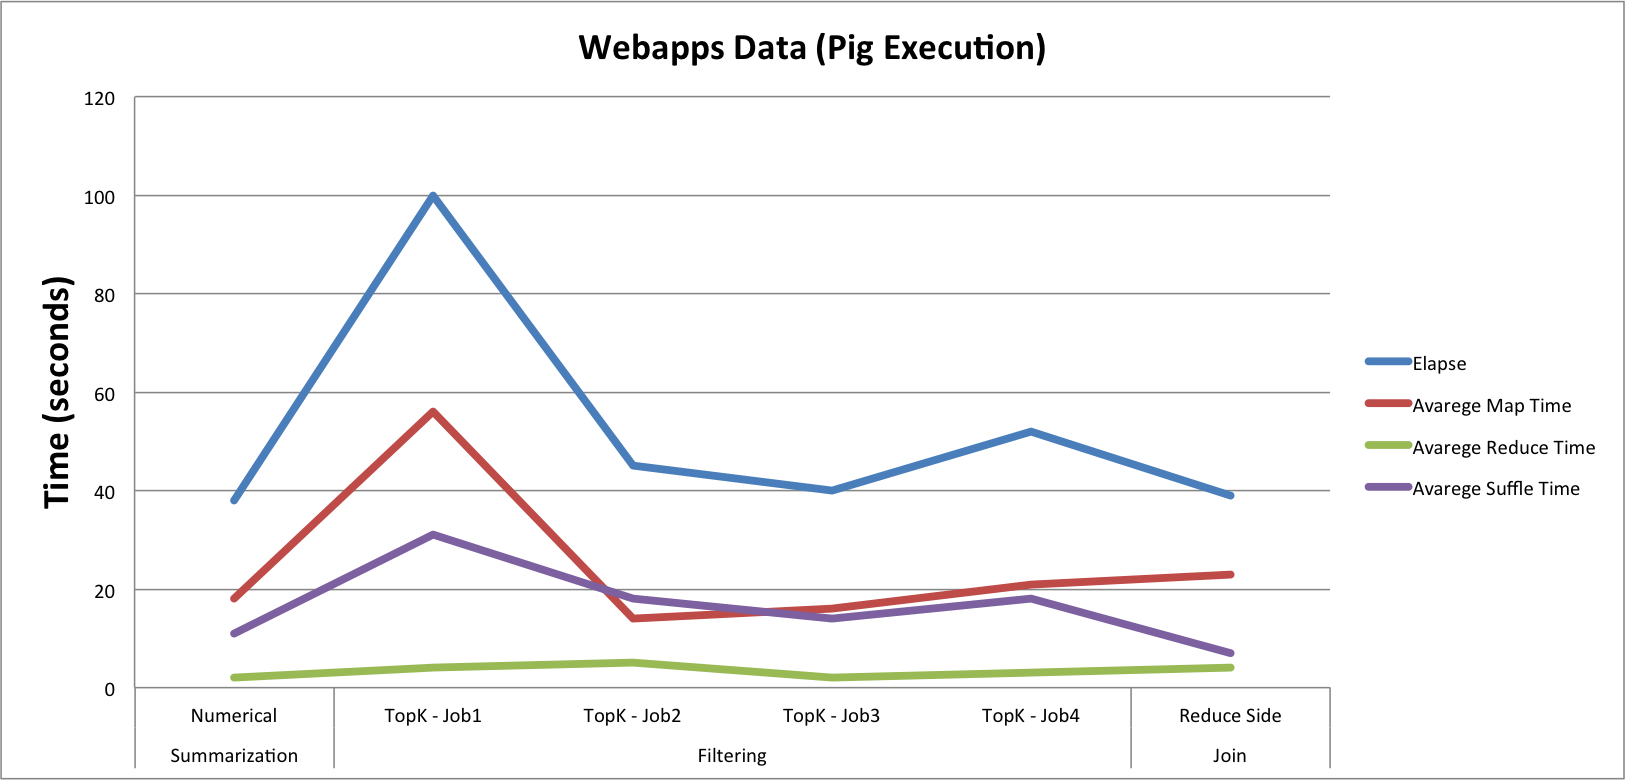
\includegraphics[width=0.5\textwidth]{figs/analysis-charts/pig/webapps.png}}
  ~ %add desired spacing between images, e. g. ~, \quad, \qquad etc. (or a blank line to force the subfig onto a new line)
 
  \caption{MapReduce Design Patterns Performance - Pig Execution.}
  \label{fig:pigexecution}
\end{figure}
     
     
\begin{figure}[ht!]
 \centering 
  \subfloat[\textit{Ebooks} Data]
  {\label{fig:pisp6}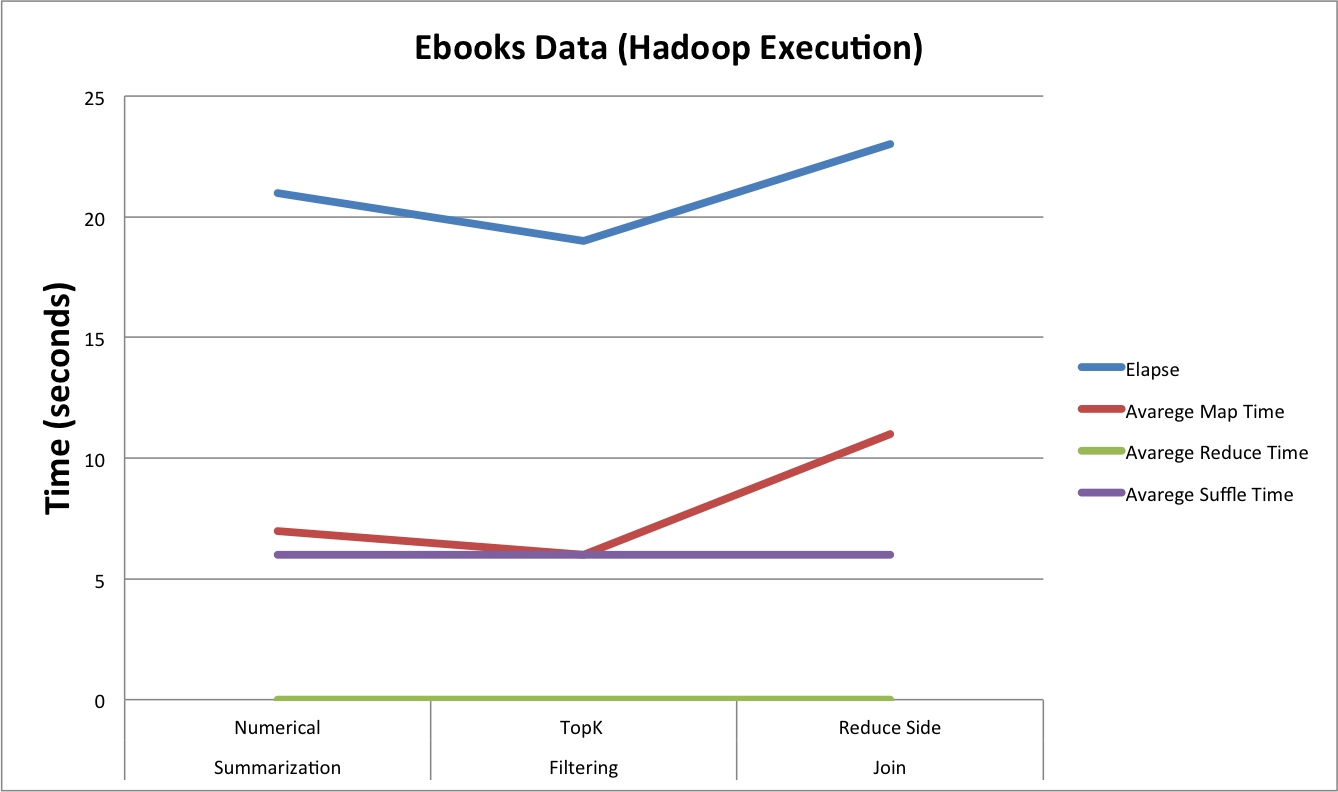
\includegraphics[width=0.456\textwidth]{figs/analysis-charts/hadoop/ebooks.png}}   
  \subfloat[\textit{Tex} Data]
  {\label{fig:pisp7}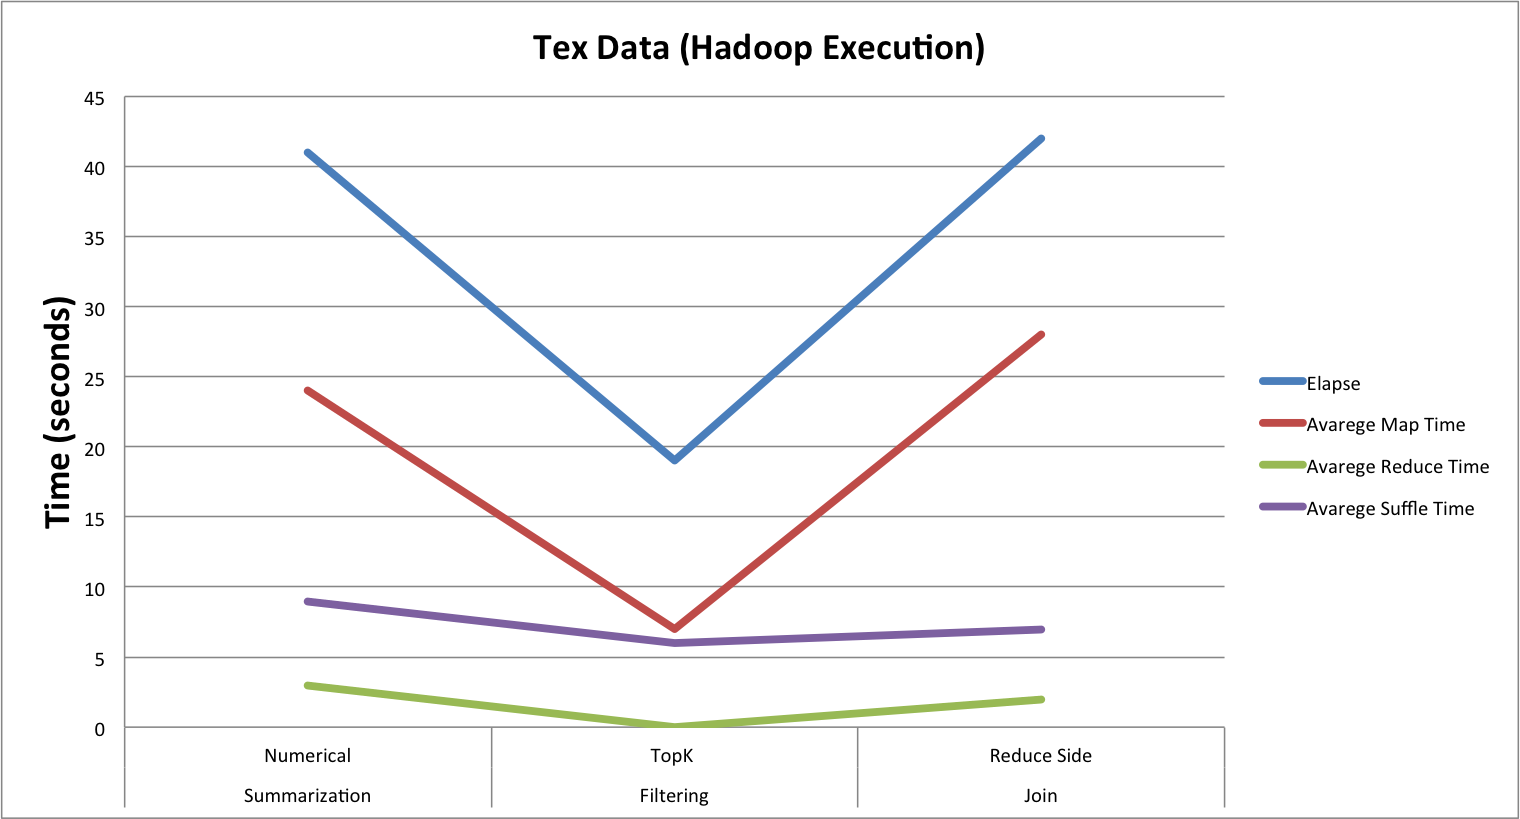
\includegraphics[width=0.5\textwidth]{figs/analysis-charts/hadoop/tex.png}}
   %add desired spacing between images, e. g. ~, \quad, \qquad etc. (or a blank line to force the subfig onto a new line)
  %~
  \\
  \subfloat[\textit{Serverfault} Data]
  {\label{fig:pisp6}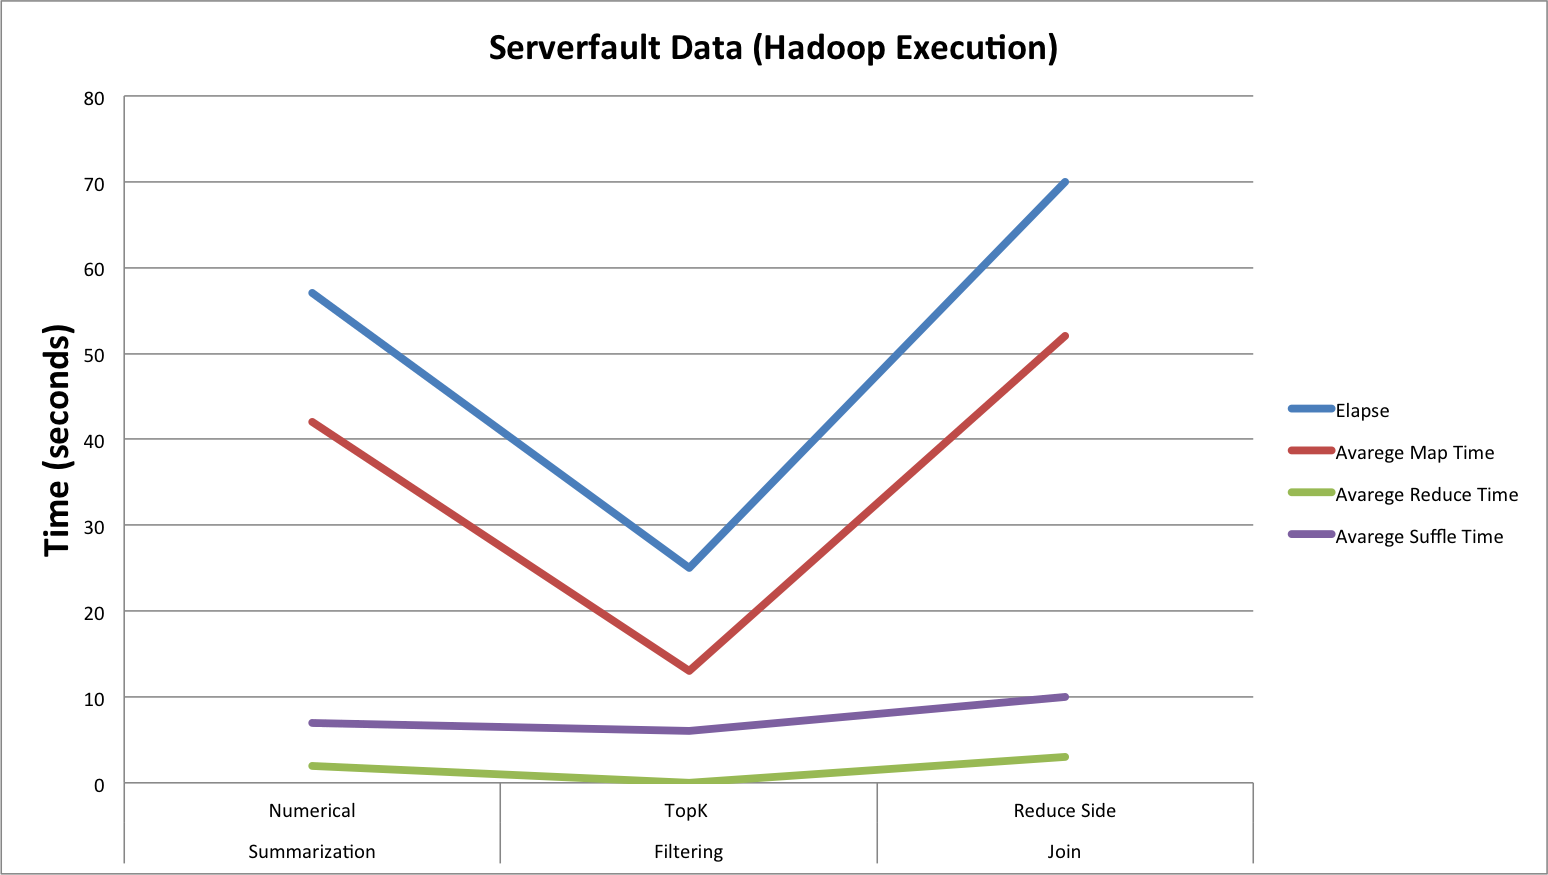
\includegraphics[width=0.485\textwidth]{figs/analysis-charts/hadoop/serverfault.png}}   
  \subfloat[\textit{Wordpress} Data]
  {\label{fig:pisp7}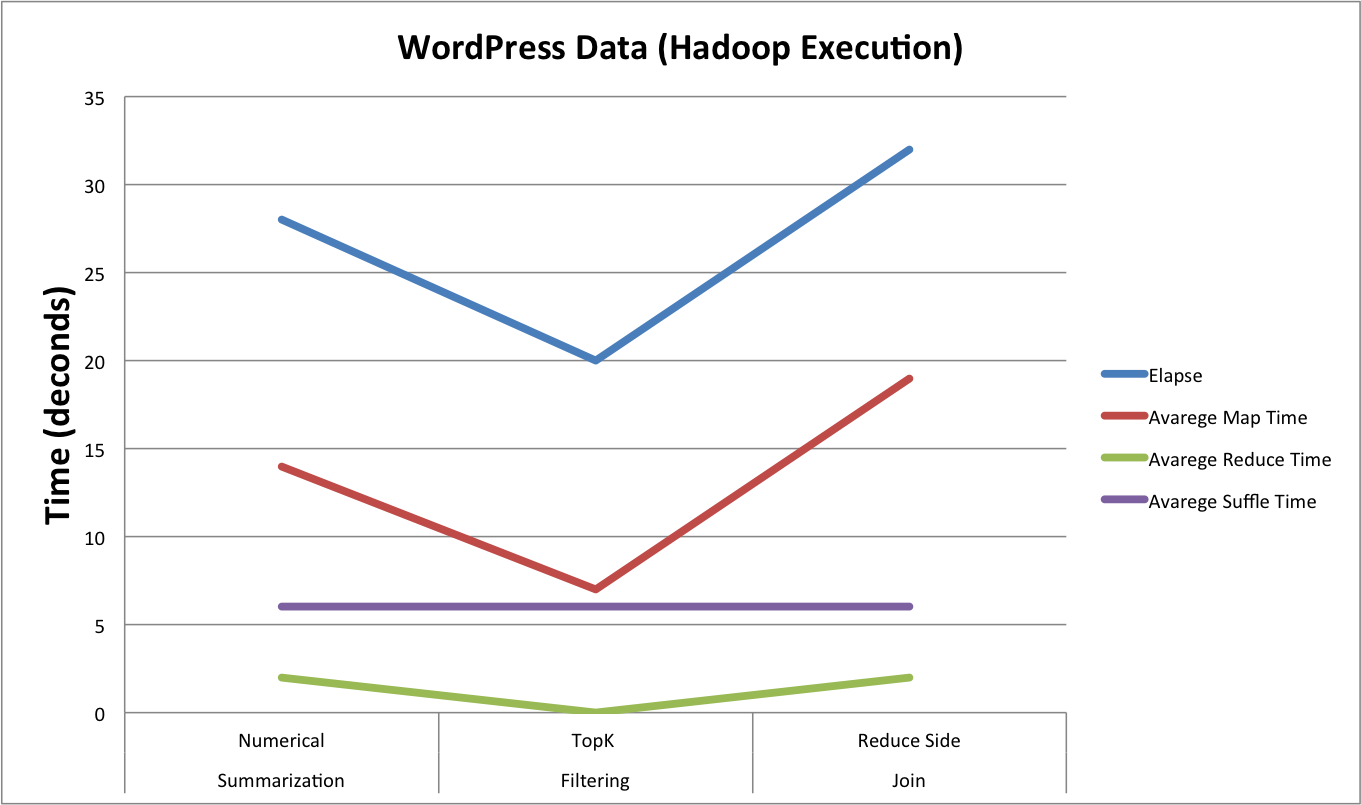
\includegraphics[width=0.466\textwidth]{figs/analysis-charts/hadoop/wordpress.png}}
   %add desired spacing between images, e. g. ~, \quad, \qquad etc. (or a blank line to force the subfig onto a new line)
  %~
  \\
  \subfloat[\textit{Webapps} Data]
  {\label{fig:pisp8}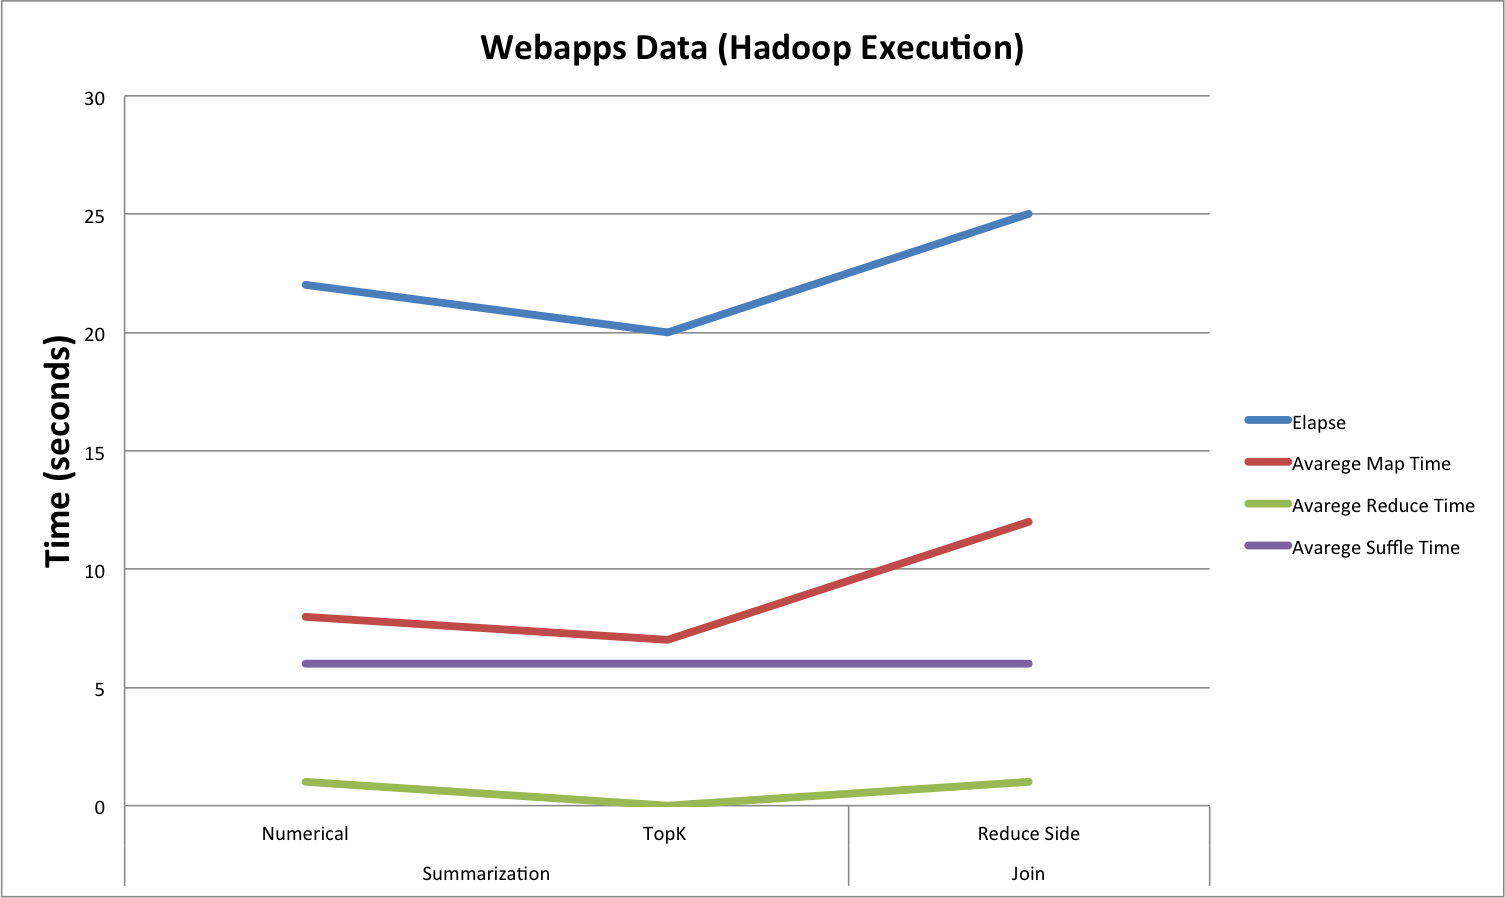
\includegraphics[width=0.5\textwidth]{figs/analysis-charts/hadoop/webapps.png}}
  ~ %add desired spacing between images, e. g. ~, \quad, \qquad etc. (or a blank line to force the subfig onto a new line)
  
  \caption{MapReduce Design Patterns Performance - Hadoop Execution.}
  \label{fig:hadoopexecution}
\end{figure}
   
   
       \begin{figure}[ht!]
 \centering 
 \subfloat[Mappers for Pig Execution]
  {\label{fig:mapperspig}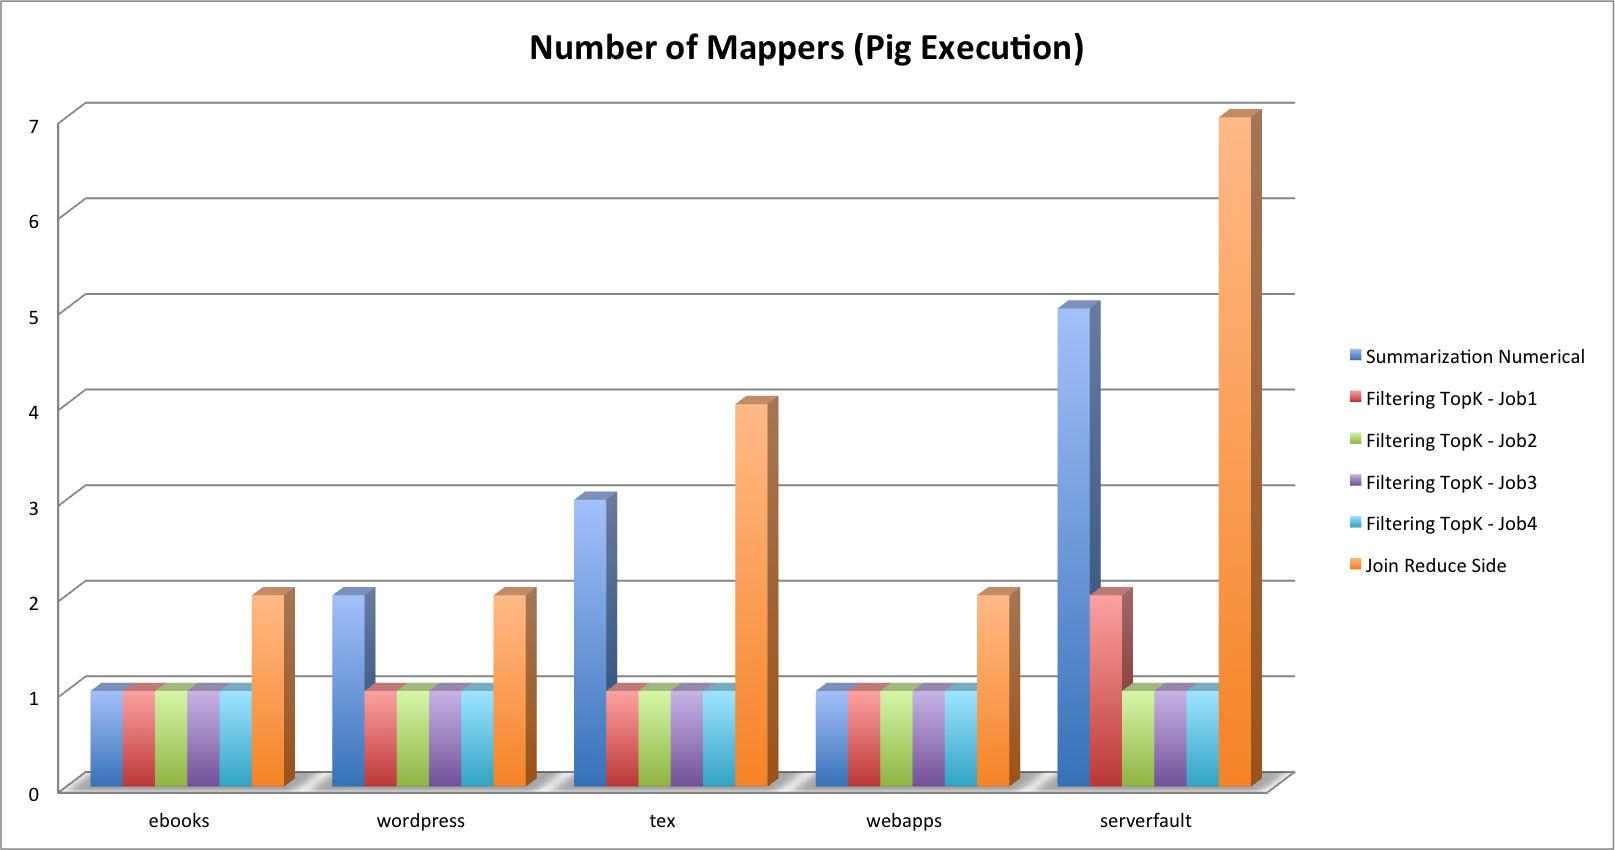
\includegraphics[width=0.6\textwidth]{figs/analysis-charts/pig/mappers.png}}
   %add desired spacing between images, e. g. ~, \quad, \qquad etc. (or a blank line to force the subfig onto a new line)
  %~
  \\
  \subfloat[Mappers for Hadoop Execution]
  {\label{fig:mappershadoop}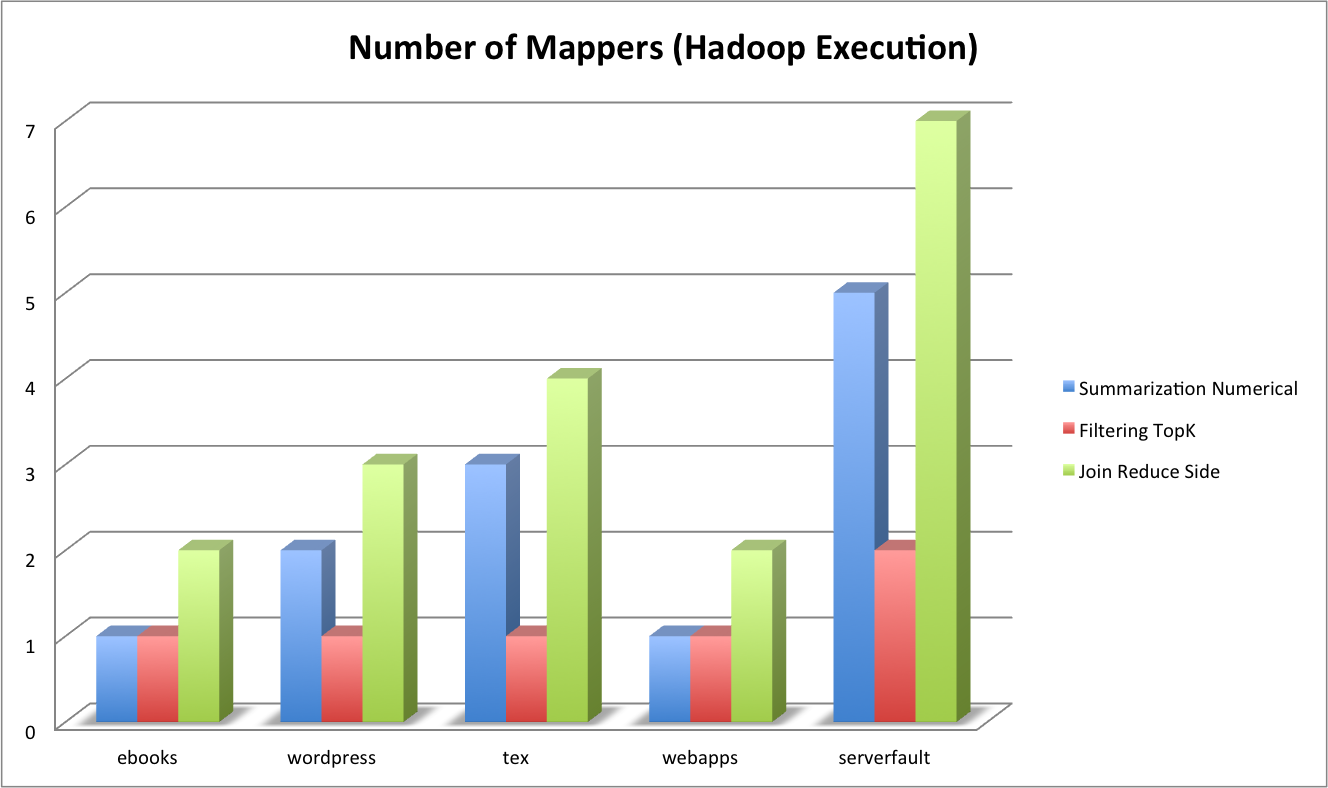
\includegraphics[width=0.6\textwidth]{figs/analysis-charts/hadoop/mappers.png}}
  ~ %add desired spacing between images, e. g. ~, \quad, \qquad etc. (or a blank line to force the subfig onto a new line)
 
  \caption{Number of Mappers - Pig and Hadoop Execution.}
  \label{fig:mappers}
\end{figure}
 
    